\chapter{Foundations} \label{ch_foundations}
\vspace{-0.45cm}
This chapter will introduce all theoretical foundations for our approach. We first introduce some notation. Then, we give an overview of the field of word equation solving, going into detail on the Nielsen transformation. Finally, we introduce some regex theories, focusing mainly on Brzozowski's work.

\section{Basics}
Words are sequences over a fixed length alphabet $\Sigma$. We write $w = w_1w_2...w_n, w_i \in \Sigma$. We denote the set of all words over $\Sigma$ as $\Sigma^*$, which forms a monoid under concatenation and the empty word $\varepsilon$. We define the length of a word $|w_1w_2...w_n| = n$.
While we use $\Sigma$ to denote the alphabet of terminal symbols, we use $X$ to denote the set of variables.
A word equation is an expression of the form $\alpha = \beta$ where $\alpha, \beta \in (\Sigma \cup X)^*$. If not specified differently, we use $a, b \in \Sigma, a \neq b$ and $x, y \in X, x \neq y$.

We define the replacement function $\varphi_{\cdot \rightarrow \cdot}(\cdot)$ so that $\varphi_{x \rightarrow \alpha}(\beta)$ denotes the result of replacing every occurrence of $x$ with $\alpha$ in $\beta$. E.g. $\varphi_{x \rightarrow ay}(xbbxy) = aybbayy$.
\[
\begin{tabular}{c c c}
    $\varphi_{x \rightarrow \alpha}(x)$ & $=$ & $\alpha$ \\
    $\varphi_{x \rightarrow \alpha}(y)$ & $=$ & $y$ \\
    $\varphi_{x \rightarrow \alpha}(a)$ & $=$ & $a$ \\
    $\varphi_{x \rightarrow \alpha}(\beta_1\beta_2...\beta_n)$ & $=$ & $\varphi_{x \rightarrow \alpha}(\beta_1)\varphi_{x \rightarrow \alpha}(\beta_2)...\varphi_{x \rightarrow \alpha}(\beta_n)$ \\
\end{tabular}
\]
Additionally, we introduce the prefix deletion function $\varphi_{DEL}$ with
\[
    \varphi_{DEL}(a\alpha) = \alpha
\]
Finally, for readability, we define the reverse order function composition $\circ'$ with
\[
    f \circ' g = g \circ f
\]

\section{Word Equations}

A word equation is an expression of the form $\alpha_1x_1\alpha_2x_2...x_{n-1}\alpha_n = \beta_1y_1\beta_2y_2...y_{m-1}\beta_m$ where $\alpha_i, \beta_i \in \Sigma^*, x_i, y_i \in X$. Now, the goal is to find out if there is an assignment function $\assignment{\cdot}: X \rightarrow \Sigma^*$ s.t. $\alpha_1\assignment{x_1}\alpha_2\assignment{x_2}...\assignment{x_{n-1}}\alpha_n = \beta_1\assignment{y_1}\beta_2\assignment{y_2}...\assignment{y_{m-1}}\beta_m \in \Sigma^*$. In other words, we are interested in finding a function that maps the variables to words in a way that makes both sides of the equation equal. Sometimes we might just be interested in finding out whether such a mapping exists without constructing it.

We consider two special cases of word equations: \textit{Quadratic} word equations and \textit{regular} word equations. Quadratic word equations are equations in which each variable occurs at most twice. For example, $xxy = ayz$ is quadratic, while $xxy = axz$ is not. Regular word equations are an even stricter subclass of quadratic word equations: Each variable may occur at most once on each side. $xy = ax$ is regular, while $xx = ay$ is not.

\section{Constrained Variables}
Until now, variables have always been \textit{unconstrained} in the way that they can take any values from $\Sigma^*$. This is not sufficient for many real-world applications. Modeling dates or passwords, for example, requires the variables to follow special formats, to have specific lengths or to be selected over only a subalphabet of $\Sigma$.

Instead of $x \in \Sigma^*$, we shall write $x \in \Sigma^k$ to denote variables whose values must be of length $k$. Similarly, we write $x \in \Sigma'^*$ for $\Sigma' \subset \Sigma$ to denote variables that only take symbols from a restricted subset of $\Sigma$.
For now, the only other kind of constraint we are interested in is regular expressions.

Let the notion $x \in ab*$ stand for the constraint that $x$ must match the regular expression $ab*$. This means $x$ can take the values $a, ab, abb, ...$ but not $b$ or $\varepsilon$. This work will focus on implementing regex constraints for variables in the Nielsen transformation. The reason for this is that regular expressions are generally expressive and that they prove powerful enough to cover most constraints presented in this chapter, albeit with drawbacks in usability or blowup in complexity. Subalphabets $\Sigma' = \{\sigma'_1, \sigma'_2, ... \sigma'_n\}$ can be modeled as one exhaustive disjunction over all terminal symbols of that subalphabet with $x \in \sigma'_1 | \sigma'_2 | ... | \sigma'_n$. This means that this simple constraint can only be modeled with linear complexity. Constant length constraints $x \in a^k$ can be modeled with $x \in \underbrace{aa...a}_{k}$. Again, we see linear blowup.
As regular languages are less powerful than context-free languages, complicated counting constraints where multiple variables depend on the same length constant $k$ cannot be modelled.

\section{Methods for Solving Word Equations} \label{methods}

To solve such equation problems, we can employ multiple different methods. This can involve manipulating the equation in various ways, such as substituting values for variables, rearranging terms, rewriting the equation in some way to simplify it or applying rules of algebra. Keep in mind that we are on a monoid, so basic tricks like adding an inverse do not work. Depending on the complexity of the equation and the methods used to solve it, solving a word equation can be a simple or a challenging task.

There are many different approaches for solving word equations, and the appropriate approach will depend on the specific problem and the requirements of the solution. Some common techniques for solving word equations include
\begin{itemize}
    \item guessing the variables by brute force
    \item guessing the variables by educated guessing
    \item simplifying the equation
    \item isolating variables
    \item fixing the position
    \item approximating lengths
    \item left side elimination
\end{itemize}

\textit{Fixing the positions} and \textit{approximating lengths} are approaches that try to approximate the variable position or length by some variation of binary search.
\textit{Left side elimination} makes use of the basic fact that string equality can be recursively defined:

\begin{definition} \label{def:string_eq}
  Let $a_1a_2...a_n, b_1b_2...b_m $ be two strings $\in \Sigma^*$.
  The recursively defined equality $a_1a_2...a_n = b_1b_2...b_m$ holds iff the prefixes $a_1$ and $b_1$ are equal and the remaining suffixes $a_2...a_n$ and $b_2...b_m$ are equal. I.e. iff $a_1 = b_1$ and $a_2...a_n = b_2...b_m$. The base case for this recursive comparison is $\varepsilon = \varepsilon$.
\end{definition}

\begin{theorem}
  The string equality defined in Definition \ref{def:string_eq} -- like other equalities -- describes an equivalence relation. The following properties hold for any $\alpha, \beta, \gamma \in \Sigma^*$:
  
  \begin{enumerate}
      \item Reflexivity: $\alpha = \alpha$
      \item Symmetry: $\alpha = \beta \Rightarrow \beta = \alpha$
      \item Transitivity: $\alpha = \beta \land \beta = \gamma \Rightarrow \alpha = \gamma$
  \end{enumerate}
\end{theorem}

\section{Nielsen Transformation}
One method for left side elimination is the Nielsen transformation \cite{nielsen1917}. It is defined for equations of terminals and unconstrained variables. It extends the recursive definition \ref{def:string_eq} of string equality for terminal words over $\Sigma^*$ to terminal and variable words over $(\Sigma \cup X)^*$ by making use of a case analysis. Keep in mind that two strings are only equal if their prefixes are equal.

Let $a, b \in \Sigma, a \neq b$ two distinct terminals, $x, y \in X, x \neq y$ two distinct variables and $\alpha, \beta \in (\Sigma \cup X)^*$ two (possibly equal) strings. Then for the Nielsen transformation, there are the following cases:

\begin{enumerate}
    \item \label{def:nt_aa}
        Both sides start with the same terminal: $a\alpha = a\beta$. \\
        We can eliminate this terminal and reduce the equality problem to $\alpha =\beta$.
    
    \item \label{def:nt_ab}
        Both sides start with a different terminal: $a\alpha = b\beta$ \\
        The strings cannot be equal, because $a \neq b$.
        
    \item \label{def:nt_xe}
        One side starts with a variable: $x\alpha = \beta$ \\
        We try to set this variable to $\varepsilon$ and check if the equation can be solved.
        
        If $x$ is empty we have to assume that every occurrence of $x$ is empty. We have to remove $x$ from both sides of the equation.

        \begin{center}
        \begin{tabular}{r c l}
            $x\alpha$ & $=$ & $\beta$ \\    
            $\varphi_{x \rightarrow \varepsilon}(x\alpha)$ & $=$ & $\varphi_{x \rightarrow \varepsilon}(\beta)$ \\
            $\varphi_{x \rightarrow \varepsilon}(\alpha)$ & $=$ & $\varphi_{x \rightarrow \varepsilon}(\beta)$
        \end{tabular}
        \end{center}

        Here, we assumed without loss of generality that the side starting with a variable is the left hand side of the equation (We may assume this because the equality relation is symmetrical).

    \item \label{def:nt_xa}
        One side starts with a variable and one starts with a terminal: $x\alpha = a\beta$
        
        This is only possible if $x$ starts with $a$ or if $x$ is empty. The case that $x$ is empty is already covered in case \ref{def:nt_xe}. Therefore, we assume that $x$ starts with $a$. If $x$ starts with $a$, we must assume that $a$ is a prefix for $x$ for every occurrence of $x$. In other words, we introduce a new variable $x'$, s.t. $x = ax'$. We then rewrite the equation:
        
        \begin{center}
        \begin{tabular}{r c l}
            $x\alpha$ & $=$ & $a\beta$ \\
            $\varphi_{x \rightarrow ax'}(x\alpha)$ & $=$ & $\varphi_{x \rightarrow ax'}(a\beta)$ \\
            $ax'\varphi_{x \rightarrow ax'}(\alpha)$ & $=$ & $a\varphi_{x \rightarrow ax'}(\beta)$ \\
        \end{tabular}
        \end{center}
        
        As introducing a new variable for each substitution quickly becomes tedious, we "recycle" the variables: Instead of replacing $x$ with $ax'$ we replace $x$ with $ax$. This is especially useful, because $xa = bx$ is isomorph to $x'a = bx'$ as we will see later. In this case, our rewrite looks like this:
        
        \begin{center}
        \begin{tabular}{r c l}
            $ax\varphi_{x \rightarrow ax}(\alpha)$ & $=$ & $a\varphi_{x \rightarrow ax}(\beta)$ \\
        \end{tabular}
        \end{center}
    
    \item \label{def:nt_xx}
        Both sides start with the same variable: $x\alpha = x\beta$ \\
        Both sides have the same prefix. We can just delete the prefix $x$. Whatever solution for $x$ solves the equation, can be determined later.
        We are thus left with $\alpha = \beta$.
        
    \item \label{def:nt_xy}
        Both strings start with different variables: $x\alpha = y\beta$ \\
        This means that one variable must be the prefix of the other variable. Without loss of generality we assume $y$ to be the prefix of $x$.
        
        \begin{center}
        \begin{tabular}{r c l}
            $x\alpha$ & $=$ & $y\beta$ \\
            $\varphi_{x \rightarrow yx}(x\alpha)$ & $=$ & $\varphi_{x \rightarrow yx}(y\beta)$ \\
            $yx\varphi_{x \rightarrow yx}(\alpha)$ & $=$ & $y\varphi_{x \rightarrow yx}(\beta)$ \\
        \end{tabular}
        \end{center}
\end{enumerate}

An equation $\alpha = \beta$ is solvable iff $\varepsilon = \varepsilon$ can be derived from repeated application of these rules.

Keep in mind that some of the cases are not necessarily exclusive and can overlap (e.g. \ref{def:nt_xe} and \ref{def:nt_xa}). Just because one case does not yield a solution does not mean another case will yield no solution either. For example $x = a$ matches the form $x\alpha = \beta$, but case \ref{def:nt_xe} cannot be used to reduce $x = a$ to $\varepsilon = \varepsilon$, instead case \ref{def:nt_xa} must be used. This must be taken into account when implementing a solver.

We can model the satisfiability problem as a graph reachability problem. Each node holds a word equation. If one word equation can be rewritten into another word equation by one of our rewrite rules, we draw a directed edge from its node to the others' node. The question whether $\alpha = \beta$ can be rewritten to $\varepsilon = \varepsilon$ is equivalent to the question whether the node holding $\varepsilon = \varepsilon$ can be reached from the node holding $\alpha = \beta$.

\begin{figure}[H]
\begin{center}
\resizebox{0.6 \textwidth}{!}{
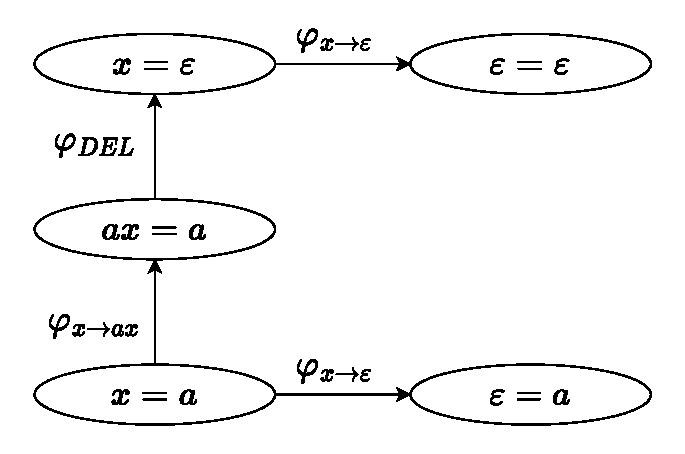
\includegraphics[]{images/x_a.pdf}
}
\caption{Graph for the satisfiable word equation $x = a$}
\label{fig:nielsen-graph-sat}
\end{center}
\end{figure}

Let us consider the simple and satisfiable word equation $x = a$. Figure \ref{fig:nielsen-graph-sat} shows the graph of the rewrites. We start at the bottom left with $x = a$. The equation can be rewritten, either by deleting $x$ and thus rewriting the equation by $\varphi_{x \rightarrow \varepsilon}$ (case \ref{def:nt_xe}), or by assuming that $a$ must be a prefix of $x$, triggering the rewrite $\varphi_{x \rightarrow ax}$ (case \ref{def:nt_xa}). In the latter case we arrive at the equation $ax = a$. We delete the prefix $a$ from both sides (case \ref{def:nt_aa}), arriving at $x = \varepsilon$. By deleting $x$ (case \ref{def:nt_xe}), we reach $\varepsilon = \varepsilon$. We reach $\varepsilon = \varepsilon$ from $x = a$ via the directed path characterized by the chain of rewrites $\varphi = \varphi_{x \rightarrow ax} \circ' \varphi_{DEL} \circ' \varphi_{x \rightarrow \varepsilon}$, because $\varphi(x) = \varepsilon = \varphi(a)$. We say $x = a$ is satisfiable with the solution $\varphi$.

\begin{figure}[H]
\begin{center}
\resizebox{0.6 \textwidth}{!}{
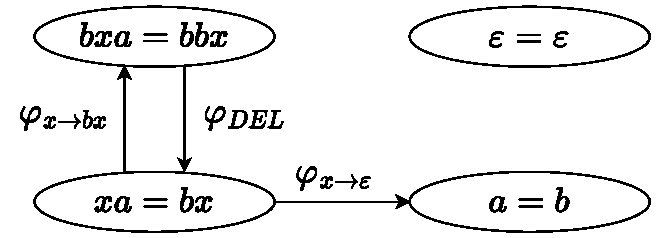
\includegraphics[]{images/xa_bx.pdf}
}
\caption{Graph for the unsatisfiable word equation $xa = bx$}
\label{fig:nielsen-graph-unsat}
\end{center}
\end{figure}

Let us now consider the case of an unsatisfiable equation: $xa = bx$ (figure \ref{fig:nielsen-graph-unsat}). We start at the bottom left and try to reach the top right node $\varepsilon = \varepsilon$. Again, we can either delete $x$ arriving at the dead end $a = b$, or we assume that $x$ has the prefix $b$. In this case we reach the equation $bxa = bbx$. We delete the shared prefix $b$ from both sides of the equation, bringing us back to $xa = bx$. No other rewrite rule applies. We cannot reach $\varepsilon = \varepsilon$. Therefore, the equation $xa = bx$ is unsatisfiable.

We reduced the satisfiability of word equations to a graph reachability problem. We can solve the reachability problem with any graph discovery algorithm. This includes depth-first search (DFS) and breadth-first search (BFS).
Interestingly, this also includes Dijkstra's \cite{dijkstra} algorithm for finding the shortest path. It generalizes BFS with a cost function. This cost function could be a heuristic, ranking each word equation by how promising it is to be reducible to $\varepsilon = \varepsilon$. Given a good cost function, Dijkstra could solve satisfiable equations faster than BFS. Note, however, that unsatisfiable equations would still take as long as with BFS, because Dijkstra's algorithm still has to perform an exhaustive graph search, if it cannot find a path. While this is an interesting idea, in this work we will not focus on finding heuristics.

To answer the question of satisfiability, we just need to find out whether some path of rewrites from $\alpha = \beta$ to $\varepsilon = \varepsilon$ exists. If we are interested in finding a satisfying variable assignment, we can backtrack over such a path. If we are interested in finding all assignments, we backtrack over all such paths.

Day et al. \cite{manea-nielsen} proved that the satisfiability problem for regular word equations is in NP and that for quadratic word equations the algorithm terminates in finite time.

This algorithm only works for unconstrained variables. In the next section we will have a look at regular expressions and how we can use them to constrain variables.

\section{Regular Expressions}
A regular expression $p$ over the alphabet $\Sigma$ describes a specific subset of $\Sigma^*$.
We use $L(p)$ to describe the set of words that are described by $p$. \cite{brzozowski}

We recursively define regular expressions to be either one of the base cases
\begin{enumerate}
    \item A symbol $a \in \Sigma$. $L(a) = \{a\}$
    \item The empty regex $\lambda$ that only matches the empty string $\varepsilon$. $L(\lambda) =            \{\varepsilon\}$
    \item The never matching regex $\emptyset$ that matches no string. $L(\emptyset) = \{\}$. This will later prove useful to model error states.
\end{enumerate}

Let $p, q$ be regular expressions over $\Sigma$. We now add the following recursive definitions to also be regular expressions

\begin{enumerate}
    \setcounter{enumi}{3}
    \item The concatenation $pq$. This matches all words $ww'$ where $w \in L(p), w' \in L(q) $
    \item The iteration $p*$. This regex matches zero or more occurrences of $p$. $L(p*) = L(\lambda) \cup L(p) \cup L(pp) \cup ...$
    \item The negation $p'$. This matches precicely when $p$ does not match. $L(p') = \Sigma^* \setminus L(p)$
    \item The conjunction $p\:\&\:q$. $L(p\:\&\:q) = L(p) \cap L(q)$
    \item The disjunction $p\:|\:q$. $L(p\:|\:q) = L(p) \cup L(q)$
\end{enumerate}

We denote the set of all regular expressions over $\Sigma$ as $R(\Sigma)$.


\subsection{Brzozowski Derivatives}
In his 1964 work, Brzozowski \cite{brzozowski} introduced a methodology for regular expression matching that does not construct an intermediary automaton. For this he defined a notion of \textit{derivatives} of a regular expression. The derivative of a regular expression $p$ respective to the symbol $a$ is the remainder of $p$ after successfully matching the first character $a$. Let us consider $a \in \Sigma, w \in \Sigma^*, p \in R(\Sigma)$. We define the derivative $D_ap$ in a way s.t. $aw \in L(p) \Leftrightarrow w \in L(D_ap)$.

Take for example the string $ab$ and the regex $a(b|c)$. To decide whether $ab \in a(b|c)$, we take the prefix of $ab$, i.e. $a$ and then calculate the derivative $D_a(a(b|c)) = b|c$. We reduced the matching problem $ab \in a(b|c)$ to $b \in b|c$. Now, we take the derivative $D_b(b|c) = \lambda|\emptyset$. We now reduced our problem to $\varepsilon \in \lambda|\emptyset$. Note that $\varepsilon \in L(\lambda) \cup L(\emptyset)$. Therefore, $ab \in a(b|c)$.

We always solve the matching problem by deriving character-by-character and then deciding whether the remaining regular expression matches $\varepsilon$:
Let $w = w_1w_2...w_n \in \Sigma^*$, then $w \in p \Leftrightarrow \varepsilon \in D_{w_n}(...(D_{w_2}(D_{w_1}p)))$. Thus, we only need a method of determining whether a regex $p$ is nullable, i.e. whether $\varepsilon \in p$. For this we define the nullability function $\nu: R(\Sigma) \rightarrow \{false, true\}$ with $\nu(p) \Leftrightarrow \varepsilon \in p$.

\[
\begin{tabular}{c c c}
    $\nu(\lambda)$ & $=$ & $true$ \\
    $\nu(\emptyset)$ & $=$ & $false$ \\
    $\nu(a)$ & $=$ & $false$ \\
    $\nu(pq)$ & $=$ & $\nu(p) \land \nu(q)$ \\
    $\nu(p*)$ & $=$ & $true$ \\
    $\nu(p')$ & $=$ & $\neg \nu(p)$ \\
    $\nu(p\:\&\:q)$ & $=$ & $\nu(p) \land \nu(q)$ \\
    $\nu(p\:|\:q)$ & $=$ & $\nu(p) \lor \nu(q)$ \\
\end{tabular}
\]

We can now define $D_ap$ as

\[
\begin{tabular}{c c l}
    $D_aa$ & $=$ & $\lambda$ \\
    $D_ab$ & $=$ & $\emptyset$ \\
    $D_a\lambda$ & $=$ & $\emptyset$ \\
    $D_a\emptyset$ & $=$ & $\emptyset$ \\

    $D_a(pq)$ & $=$ & $
    \left\{
	\begin{array}{ll}
		(D_ap)q\:|\:D_aq  & \mbox{if } \nu(p) \\
		(D_ap)q & \mbox{if } \neg \nu(p)
	\end{array}
    \right.
    $ \\
    
    $D_a(p*)$ & $=$ & $(D_ap)p*$ \\
    $D_a(p')$ & $=$ & $(D_ap)'$ \\
    $D_a(p\:\&\:q)$ & $=$ & $D_ap\:\&\:D_aq$ \\
    $D_a(p\:|\:q)$ & $=$ & $D_ap\:|\:D_aq$ \\
\end{tabular}
\]

Brzozowski also presented an algorithm to construct a DFA from a regular expression.
Brzozowski's notion of derivatives inspired an entire field of research and regex theories. In the following sections we will touch on two of these.

\subsection{Antimirov Derivatives}
In his 1995 work, Antimirov \cite{antimirov} introduced the notion of \textit{partial derivatives}. Just like Brzozowski's derivatives can be used to construct a DFA, Antimirov's partial derivatives can be used to construct an NFA. Antimirov does this by defining the partial derivative of $p$ respective to $a$ as $\partial_a : R(\Sigma) \rightarrow 2^{R(\Sigma)}$ as opposed to Brzozowski's $D_a : R(\Sigma) \rightarrow R(\Sigma)$. Antimirov also presents an algorithm for constructing a DFA that is more compact than Brzozowki's. 

\subsection{Transition Regexes}
Stanford et al. \cite{transition-regex} present the notion of \textit{symbolic derivatives}. Instead of operating on a regex, they return functions that later evaluate to regexes. By doing this, they delay branching and decision making for as long as possible. In their benchmarks they outperform Brzozowski derivatives and perform especially well on regular expressions with logical branches ($\&$ and $|$).

Both of these approaches are complete regex theories and can be used for regex matching. In this work, to keep it simple, we will only focus on the classic Brzozowski derivatives. In the next chapter, we will describe how to incorporate them into the Nielsen transformation.